\documentclass{beamer}
%\usetheme{Madrid}
%\usepackage[pdftex]{graphicx}
%\usepackage{sidecap}
\usepackage{wrapfig}
\graphicspath{{../resources/}}
\title{Software Patents}
\author{Tom Augspurger \& Caleb Floyd}
\date{\today}

\begin{document}
\frame{\titlepage}

\begin{frame}
	\frametitle{Copyright Term Extension Act}
  \begin{itemize}
    \item CTEA of 1998
	  \begin{itemize}
		\item Created prior to 1978: 95 year protection
		\item Created after 1978: lifetime of the author plus 70 years
		\item Challenged on grounds of
		\begin{itemize}
			\item Copyright Clause -- "limited Times"
			\item The First Amendment
			\item The public trust doctrine
		\end{itemize}
		\item Upheld in \emph{Eldred v. Ashcroft} by SCOTUS (January 15th, 2003)
	\end{itemize}
  \end{itemize}
\end{frame}

\begin{frame}
 \frametitle{Diamond v. Diehr (1981)}
 \begin{itemize}
	 \item Prior to 1981 software was effectively not patentable 
	 \item Mathematical formulas in the abstract are not eligible for patent protection
	 \item However, a physical machine or process which makes use of a mathematical algorithm is different from an invention which claims the algorithm in the abstract
	 \item Hence software is deemed patentable as it's an implementation of an algorythm
 \end{itemize}
\end{frame}

\begin{frame}
	\frametitle{Amazon One-Click Patent}
  \begin{columns}[T]
    \begin{column}{.5\textwidth}
	\begin{block}{}
	\tiny A method and system for placing an order to purchase an item via the Internet. The order is placed by a purchaser at a client system and received by a server system. The server system receives purchaser information including identification of the purchaser, payment information, and shipment information from the client system. The server system then assigns a client identifier to the client system and associates the assigned client identifier with the received purchaser information. The server system sends to the client system the assigned client identifier and an HTML document identifying the item and including an order button. The client system receives and stores the assigned client identifier and receives and displays the HTML document. In response to the selection of the order button, the client system sends to the server system a request to purchase the identified item. The server system receives the request and combines the purchaser information associated with the client identifier of the client system to generate an order to purchase the item in accordance with the billing and shipment information whereby the purchaser effects the ordering of the product by selection of the order button.
    \end{block}
	\end{column}
	\begin{column}{.5\textwidth}
	\begin{block}{}
	  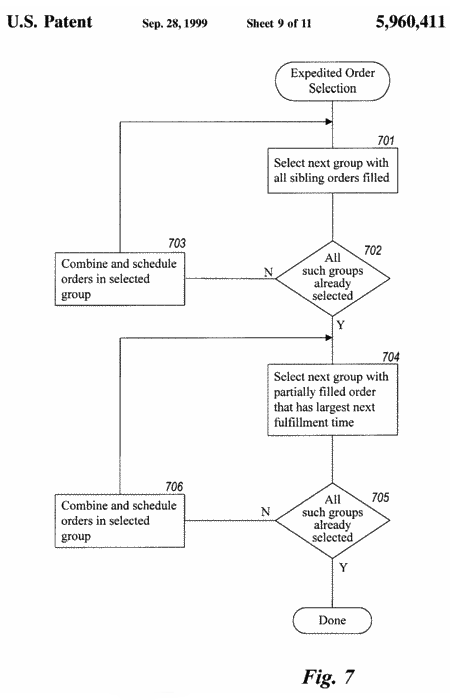
\includegraphics[height=2.75in,angle=0]{Amazon.png}
    \end{block}
	\end{column}
	\end{columns}
\end{frame}


\begin{frame}
  \frametitle{Why does open source coexist?}
  \begin{itemize}
    \item control over product performance
    \item hobbyists/enthusiasts
    \item display of skill/resume padding
	\begin{itemize}
		\item Hall et. al
	\end{itemize}
	\item competitive rents (Boldrin \& Levine)
	\begin{itemize}
		\item Which model version fits?
		\item What can we say about the implications? 
	\end{itemize}
  \end{itemize}
\end{frame}

\begin{frame}
  \begin{quotation}
    The evidence (and the common sense of anyone involved with OS software) shows   that the source of competitive rents is the complementary sale of expertise.
  \end{quotation}
  \begin{quotation}
	  ...only small rents can be obtained through the sale of copies. [Purchasers] also have a demand for services, ranging from support and consulting to customization. They naturally prefer to hire the creators of the programs who in the process of writing the software have developed specialized expertise that is not easily matched by imitators.
  \end{quotation}
  - Boldrine \& Levine (2009)
\end{frame}

\begin{frame}
  \frametitle{Boldrin \& Levine}
  Boldrin \& Levine: alternate notation\\
  \begin{table}[ht]
    \caption{Alternate Notation}
    \centering
	\begin{tabular}{c c c}
	  \hline\hline
      BL &  & New\\ [0.5ex] 
	  \hline
	  \delta & \longrightarrow & \beta  \\ 
	  \beta & \longrightarrow & \lambda \\
	  \zeta & \longrightarrow & $1 - \delta$ \\[1ex] 
	  \hline
	 \end{tabular}
	 \label{table:altnot}
  \end{table}
\end{frame}

\begin{frame}
  \frametitle{Boldrin \& Levine: General Model Revisited}
  \begin{itemize}
    \item Distinguish between productive input and consumption good: $\{k,c\}$
	\item $c_t = F(k_t^c,l_t^c)$, $x_t = G(k_t^k,l_t^k)$
	\item Agent solves $\displystyle\sum\limits_{t=0}^\infty\beta^t[u(c_t)-wL_t]$
	\begin{itemize}
	  \item $\lambda k_t$ units available tomorrow without allocating 			resources for production: $k_{t+1} = \lambda k_t + x_t$
	  \item $\lambda > 1$ gives us the $24/7$ case
	\end{itemize}
  \end{itemize}
\end{frame}

\begin{frame}
	\frametitle{}
  \begin{itemize}
    \item Given $\{k_t, x_t, L_t\}$, the solution $c_t = T(k_t,x_t,L_t)$ traces a 		 production possibility frontier\\
	   graph here
	\item $L_t$ solves $\underset{L_t}{max}$ $u[T(k_t,x_t,L_t)]-wL_t$
	\item The problem restated:\\
	\begin{centering}
	  $\nu(k_0)=
		\underset{\{k_t\}_{t=1}^\infty}{max}\displystyle\sum\limits_{t=0}^\infty\beta		 ^tV(k_t,k_{t+1} - \lambda k_t)$\\
	    \hspace{13mm}
		s.t. $\lambda k_t + \overline{x}(k_t) \ge k_{t+1} \ge \lambda k_t$
	\end{centering}
	\item As before, $q_0 = \nu ' (k_0) > 0$ yields positive competitive rents
  \end{itemize}	
\end{frame}



\end{document}
